\section{Method}
\label{sec:method}

TRAIL learns a task-relevant latent change predictor from action-free human videos and uses the predicted change as policy context. During pre-training, a language-grounded encoder and an asymmetric predictor learn to forecast frozen DINOv3 future tokens from Kinetics videos without robot actions (Sec. XX). During downstream imitation learning, the retained intent stream produces a latent residual that conditions the policy for XXX (Sec. XX). 


\begin{figure*}[t]
\centering
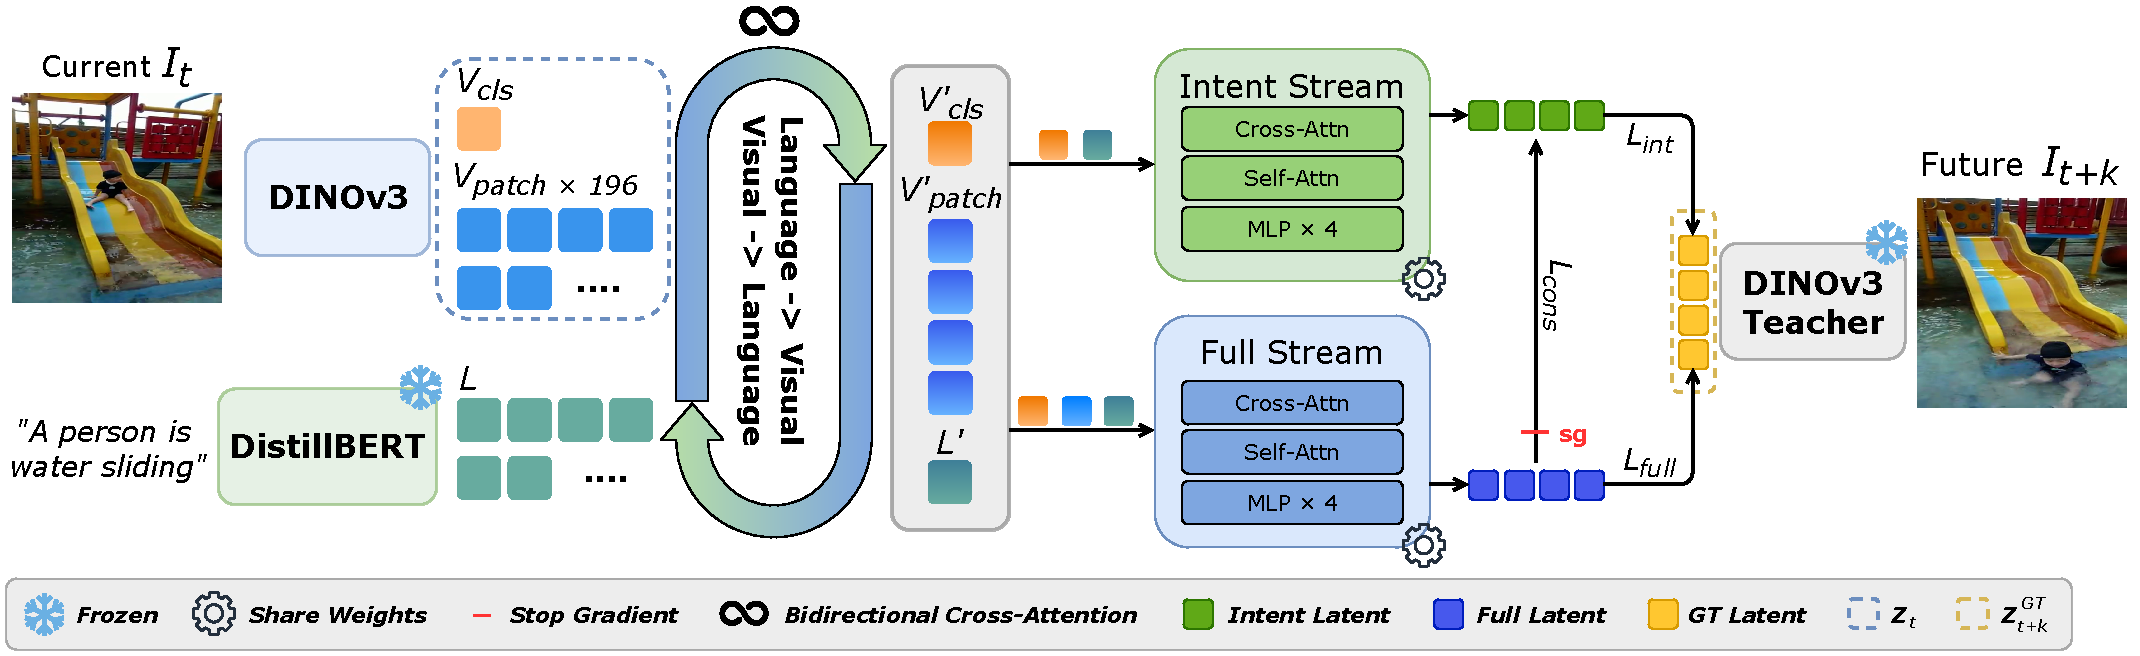
\includegraphics[width=\textwidth]{ieeeconf/figure/DiPredict_cropped.pdf}
\caption{\textbf{TRAIL architecture}. Snowflakes mark frozen modules; all other modules are trained. Visual and language tokens are first fused by bidirectional cross-attention. The same predictor is then evaluated under two memory-access conditions: the full-information stream reads class, patch, and language tokens, whereas the intent stream reads only the class and language tokens. Both streams predict the frozen future target, and the full-information prediction provides a stopped consistency target for the intent prediction. At deployment, only the intent stream is retained to produce the latent forecast used to compute $\Delta_z$.}
\label{fig:ab_probe}
\end{figure*}

\subsection{Language-guided asymmetric prediction}
\label{subsec:pretrain}
% \CO{Make this section have a following order: formulation, encoding, prediction, losses.}

% \CO{Make this section have a following order: formulation, encoding, prediction, losses.}


%

Fig.~\ref{fig:ab_probe} shows the pipeline of our pre-training, i.e. learning by language-guided asymmetric prediction. Given a current frame $I_t$, a future frame $I_{t+k}$ at frame offset $k$, and a language instruction $l$, TRAIL learns to predict the future latent target $z^{\mathrm{gt}}_{t+k}$ from the current latent $z_t$ and $l$. To disentangle task-relevant future changes from general visual dynamics, our model predicts the same future target with different levels of visual access. In particular, the full stream has access to both global and dense visual information, while the intent stream is restricted to global visual and language context. Both streams are supervised by the same future latent target, with the full prediction further guiding the intent prediction through consistency learning.

We first use a trainable visual encoder~\cite{simeoni2025dinov3} to map $I_t$ to the visual-token sequence $z_t$, while a frozen copy of the encoder maps $I_{t+k}$ to the supervision target $z^{\mathrm{gt}}_{t+k}$. At an input resolution of $224\times224$, each visual sequence contains one class token $V_\texttt{cls}$ and 196 patch tokens $V_\texttt{patch}$. A frozen DistilBERT encoder~\cite{sanh2019distilbert} maps the instruction $l$ to the language-token sequence $L$. The visual tokens, $V_\texttt{cls}$ and $V_\texttt{patch}$, and $L$ are then fused through bidirectional cross-attention. The visual tokens first query $L$ with a residual connection, producing the instruction-conditioned class token $V'_{\texttt{cls}}$ and patch tokens $V'_\texttt{patch}$. The language tokens subsequently query these updated visual tokens, producing the scene-conditioned language tokens $L'$. The class token provides a compact task-conditioned representation, while the patch tokens preserve dense spatial information.

% \subsection{\CO{Latent Space}}
% \label{subsec:notation}

% TRAIL defines current and future states in the same frozen feature space. A frozen DINOv3 visual encoder~\cite{simeoni2025dinov3} maps the current RGB frame to the token sequence $z_t$ and the future frame to the stopped training target $z^{\mathrm{gt}}_{t+k}$, where the superscript $\mathrm{gt}$ denotes ground truth. A frozen DistilBERT encoder~\cite{sanh2019distilbert}, followed by a trainable projection to the visual feature width, maps the instruction to language tokens. At $224\times224$ resolution, each visual sequence contains one class token and $N=196$ patch tokens. Throughout the paper, \texttt{[CLS]} refers only to this visual class token. The offset $k$ is a web-video pre-training gap, not a robot control horizon.

% This latent-space formulation is distinct from latent action models, which make action-free video usable for policy pre-training by \emph{inventing} an action space. An inverse dynamics model infers a latent action $u_t$ from a pair of observations $(o_t, o_{t+k})$, a forward model is asked to reconstruct $o_{t+k}$ from $(o_t, u_t)$, and a low-capacity bottleneck on $u_t$ forces it to carry the controllable part of the transition~\cite{schmidt2024learning, bruce2024genie, ye2025latent}. A policy is then pre-trained to emit $u_t$ on unlabelled video, and a small action-labelled set aligns the latent actions with real commands. The same recipe has recently been scaled to large robot corpora, where a generalist policy is pre-trained on latent actions before being grounded in real commands~\cite{agibot2025world}.

% TRAIL shares the premise that action-free video contains usable dynamics, but not the mechanism. We do not learn an action variable at all: the quantity we extract, $\Delta_z$ (Eq.~\ref{eq:residual}), lives in the observation space of a frozen perceptual encoder and is consumed by the policy as a conditioning feature, so no latent-to-real action alignment stage is required. Three differences follow. \emph{(i) Where the capacity constraint is placed.} Latent action models constrain the \emph{action} variable $u_t$ so that it captures controllable rather than passive change; the constraint is unsupervised, and the resulting variable is identified only up to a reparameterisation. TRAIL instead constrains the \emph{visual memory access}: the intent stream retains the language-grounded visual class token and contextualized language tokens but has no direct access to dense patch tokens. This capacity limit forces compression, while language grounding determines which information is emphasized. \emph{(ii) Cross-embodiment transfer.} A latent action inferred from human hands in web video is defined relative to the human embodiment, and transferring it to a parallel-jaw gripper requires the alignment stage to absorb that mismatch. A state residual carries no embodiment: it is a direction in a perceptual space shared by both, which is what allows TRAIL to pre-train on Kinetics and deploy on a robot without any in-domain robot data. \emph{(iii) How dynamics are learned without latent-action supervision.} The supervision is the prediction task itself. The model must map the current observation and the instruction onto the frozen-encoder embedding of a future frame, so $\Delta_z$ is exactly the $k$-step transition that the instruction implies. TRAIL does not need to identify \emph{which command} produced that transition, because the downstream policy is trained with real action labels; the residual only has to indicate where the scene should go, not what to send to the controller.

% The trade-off is explicit. Because $\Delta_z$ is not an action, it cannot be rolled out for planning or used as a policy target on its own, which latent action models can do. TRAIL is therefore complementary to that line of work: it is a representation-side prior rather than a substitute for the action space.

% \subsection{Language-Grounded Visual Encoding}
% \label{subsec:encoder}

% The first module grounds the current visual state in the instruction before future prediction. The visual tokens first query the language tokens through cross-attention with a residual connection, making both the class and patch tokens instruction-conditioned. The language tokens then query these updated visual tokens, incorporating the current scene into the language context. We denote the resulting visual class token by $v'_{\texttt{cls}}$, the sequence of $N$ visual patch tokens by $v'_{1:N}$, and the contextualized language-token sequence by $L'$; the prime marks tokens after language--vision fusion. The visual class token provides a compact task-relevant summary, while the patch tokens preserve dense spatial evidence.

% \subsection{Asymmetric Full and Intent Prediction}
% \label{subsec:pretraing}

%  The second module separates task-relevant future prediction from generic video extrapolation. TRAIL evaluates the same predictor under two memory-access conditions. Let $P$ denote the shared predictor and $Q$ its $N{+}1$ learned, content-free future queries. The two passes are

% \begin{align}
% \hat z^{\mathrm{full}}_{t+k}
%     &=P\!\left(Q\mid[V'_{\texttt{cls}},V'_{\texttt{cls}},L']\right), \label{eq:full_stream}\\
% \hat z^{\mathrm{int}}_{t+k}
%     &=P\!\left(Q\mid[V'_{\texttt{cls}},L']\right). \label{eq:int_stream}
% \end{align}

% Here $\hat z^{\mathrm{full}}_{t+k}$ and $\hat z^{\mathrm{int}}_{t+k}$ are the two predicted future-token sequences; $t$ is the current-frame index, $k$ is the pre-training frame offset, and the superscripts identify the full-information and intent streams. $P$ is the shared predictor, and $Q$ is its sequence of $N{+}1$ learned future queries. The terms $V'_{\texttt{cls}}$, $V'_{\texttt{patch}}$, and $L'$ are respectively the language-grounded visual class token, the $N$ dense visual patch tokens, and the contextualized language tokens defined above. The brackets denote the memory supplied to $P$, and the vertical bar separates its queries from that memory. Thus, Eq.~\ref{eq:full_stream} receives class, patch, and language tokens, whereas Eq.~\ref{eq:int_stream} receives only class and language tokens, with no direct dense-patch access. Both streams share $P$ and $Q$ and emit the same number of future tokens; only their input memory differs.


With the language-grounded tokens $V'_{\texttt{cls}}$, $V'_{\texttt{patch}}$,
and $L'$, we then perform asymmetric future prediction. The intent stream predicts the full future token sequence $z^{\mathrm{gt}}_{t+k}$ using only the instruction-conditioned class token $V'_{\texttt{cls}}$ and language tokens $L'$, without direct access to the current patch tokens $V'_{\texttt{patch}}$. To provide additional supervision during pre-training, we introduce a full-information stream that also accesses $V'_{\texttt{patch}}$. The two streams share the predictor $P$ and future queries $Q$, differing only in their memory inputs:
%
\begin{align}
\hat z^{\mathrm{full}}_{t+k}
&=P\!\left(Q\mid[V'_{\texttt{cls}},V'_{\texttt{patch}},L']\right),
\label{eq:full_stream}\\
\hat z^{\mathrm{int}}_{t+k}
&=P\!\left(Q\mid[V'_{\texttt{cls}},L']\right).
\label{eq:int_stream}
\end{align}
%
Both predictions are supervised by $z^{\mathrm{gt}}_{t+k}$. In addition, the stopped full-information prediction regularizes the intent prediction, encouraging the compact intent representation to preserve future-relevant information that is consistent with the detailed current scene. The full-information stream is used only during pre-training, and downstream policy learning retains only the intent stream.

Finally, we optimize both prediction streams by introducing three losses, the full prediction loss, the intent prediction loss, and the consistency loss as follows:
%
\begin{equation}
\mathcal{L}_{\mathrm{full}}=d\!\left(\hat z^{\mathrm{full}}_{t+k},z^{\mathrm{gt}}_{t+k}\right), \label{eq:loss_full}
\end{equation}
%
\begin{equation}
\mathcal{L}_{\mathrm{int}}=d\!\left(\hat z^{\mathrm{int}}_{t+k},z^{\mathrm{gt}}_{t+k}\right), \label{eq:loss_int}
\end{equation}
%
\begin{equation}
\mathcal{L}_{\mathrm{cons}}
=
\operatorname{MSE}\!\left(
\hat z^{\mathrm{int}}_{t+k},
\operatorname{sg}\!\left(\hat z^{\mathrm{full}}_{t+k}\right)
\right),
\label{eq:loss_cons}
\end{equation}
%
where $d(x,y)=\operatorname{MSE}(x,y)+1-\operatorname{cos}(x,y)$ is the sum of mean-squared error and cosine distance between two aligned token sequences $x$ and $y$. In Eqs.~\ref{eq:loss_full} and~\ref{eq:loss_int}, $\mathcal{L}_{\mathrm{full}}$ and $\mathcal{L}_{\mathrm{int}}$ measure the prediction errors of the full-information and intent streams with respect to $z^{\mathrm{gt}}_{t+k}$. In Eq.~\ref{eq:loss_cons}, $\mathcal{L}_{\mathrm{cons}}$ encourages the intent prediction to agree with the patch-informed full-information prediction, while $\operatorname{sg}(\cdot)$ stops gradients through the full-information output. The overall pre-training loss becomes
%
\begin{equation}
\mathcal{L}_{\mathrm{total}}
=\mathcal{L}_{\mathrm{full}}
+\mathcal{L}_{\mathrm{int}}
+\alpha\mathcal{L}_{\mathrm{cons}},
\label{eq:total}
\end{equation}
%
where $\alpha$ weights the consistency loss, empirically set to $\alpha=0.3$. 
Since $\operatorname{sg}(\cdot)$ is applied to the full-information prediction, gradients from $\mathcal{L}_{\mathrm{cons}}$ propagate only through the intent branch. The future-frame visual encoder and language encoder are frozen, while the current-frame visual encoder, language projection, fusion module, future queries, and asymmetric predictor are trainable.



\subsection{Residual-guided policy learning}
\label{subsec:policy_learning}


After pre-training, we keep only the intent stream and use its predicted future latent to construct a task-relevant residual for downstream policy learning. Given the current observation and instruction, the intent stream produces $\hat z^{\mathrm{int}}_{t+k}$ in the same frozen visual feature space as $z_t$. We then form the token-wise residual
%
\begin{equation}
    \Delta_z = \hat z^{\mathrm{int}}_{t+k}-z_t, \label{eq:residual}
\end{equation}
where $\Delta_z$ represents the task-relevant change from the current latent state. Unlike an absolute future feature, this representation makes the difference between current and predicted states explicit rather than leaving the policy to infer that difference implicitly.


% $\hat z^{\mathrm{int}}_{t+k}
% $ is the intent-stream forecast at the current control step, and $z_t$ is the current visual-token sequence. The residual exposes the predicted change from the current latent state, so the policy receives both where the scene is now and how the intent stream expects it to change. Unlike an absolute future feature, this representation makes the difference between current and predicted states explicit rather than leaving the policy to infer that difference internally.


As $\Delta_z$ can have a smaller magnitude than the current-state features, we normalize the two token sequences independently before policy readout. This prevents a simple scale difference from suppressing the residual during fusion.\CO{ Behavioral cloning [????]} then predicts the action from the balanced state and residual features together with proprioception. Low-dimensional control uses a vector readout, whereas spatial affordance policies use a patch-map readout. Table~\ref{tab:ablation_residual} compares this residual context with the current state alone, the predicted future alone, and the absolute current--future pair. Fig.~\ref{fig:acdino} illustrates the overview of the proposed policy learning.

\begin{figure}[t]
\centering
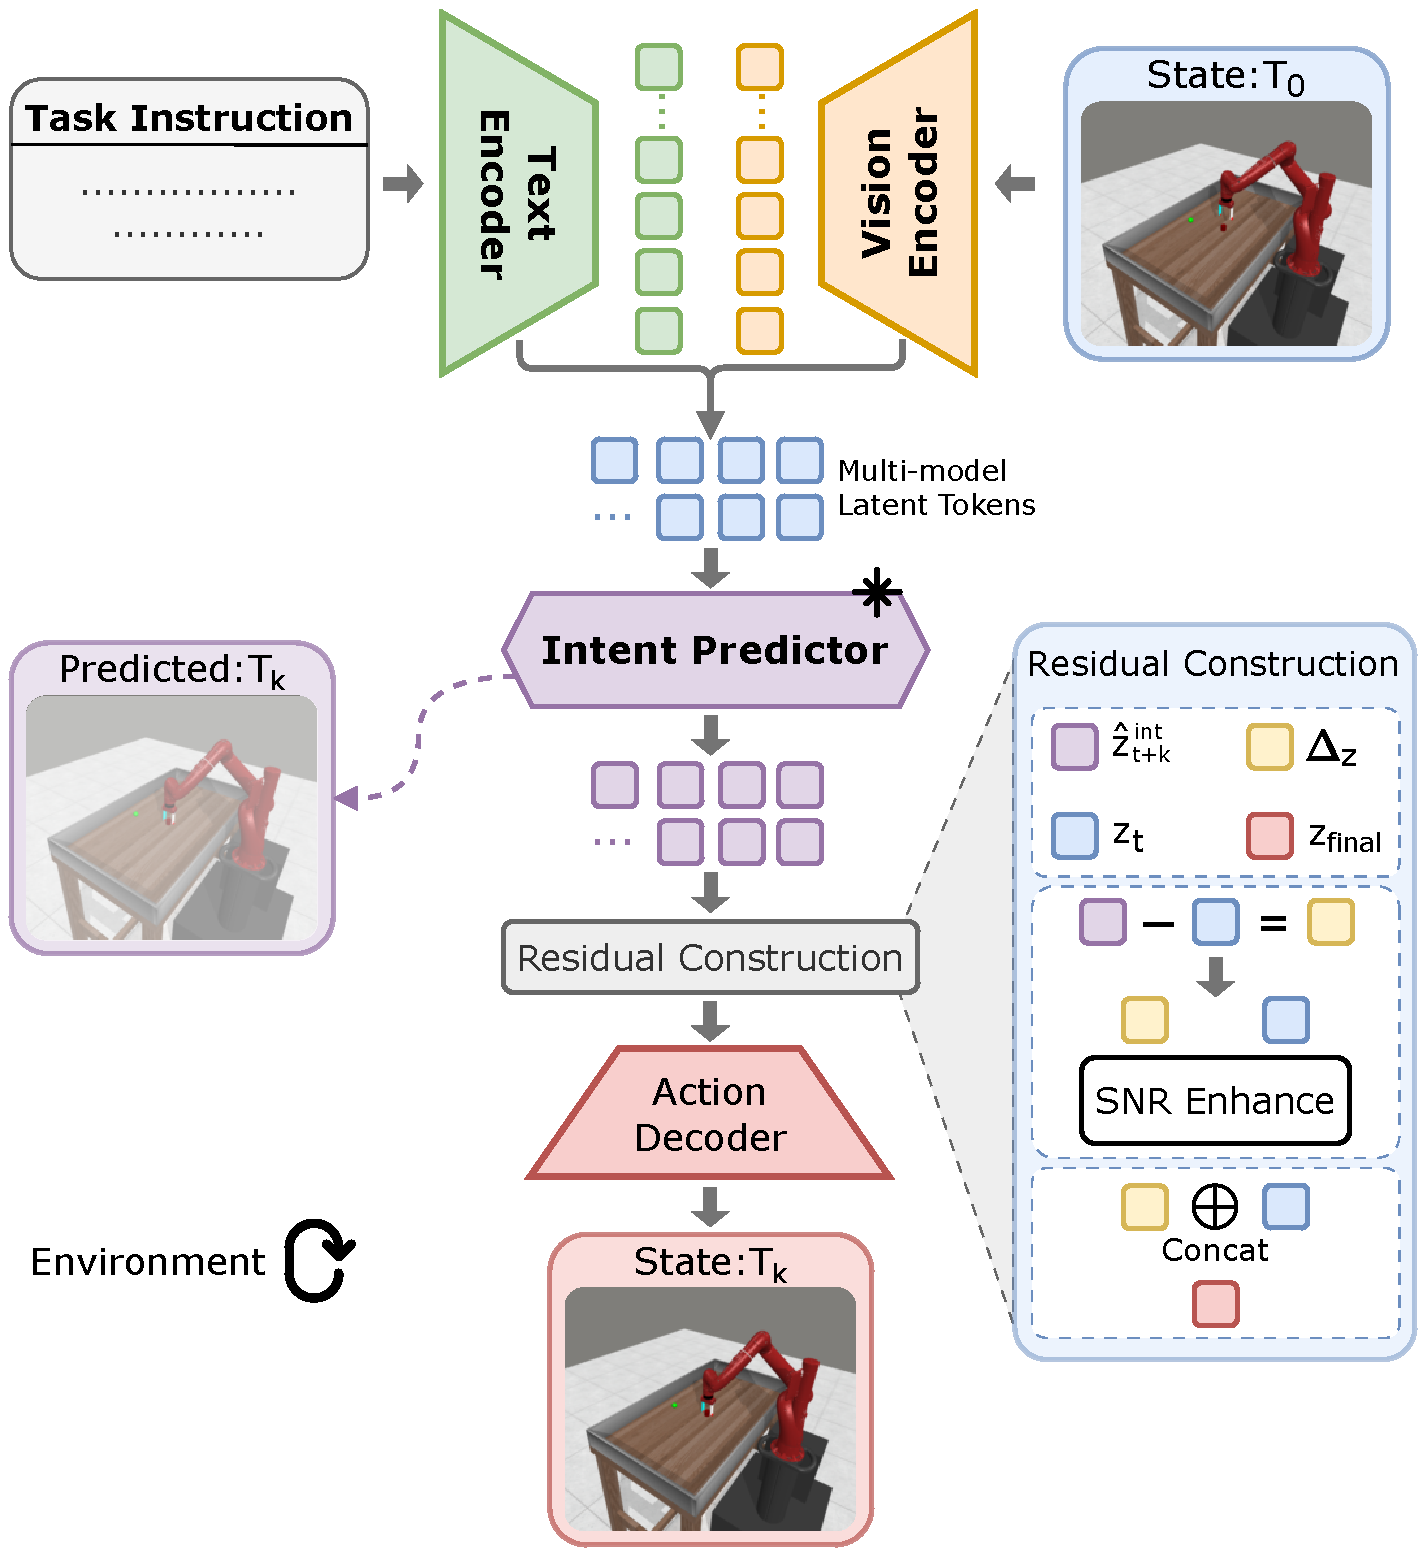
\includegraphics[width=0.95\linewidth,]{ieeeconf/figure/ACDINO_cropped}
\caption{\textbf{Proposed residual-guided policy learning}. The retained intent stream estimates a task-relevant latent forecast from the current observation and instruction. TRAIL subtracts the current latent state to obtain $\Delta_z$, balances the state and residual feature scales, then fuses them with proprioception for behavioral cloning.}
\label{fig:acdino}
\end{figure}

At deployment, the intent stream is executed at every control step in closed loop. Given the current image and instruction, the model predicts $\hat z^{\mathrm{int}}_{t+k}$ and computes $\Delta_z$, and then predicts an action. This process is repeated after each robot action, and the predictor is not rolled out over multiple future steps. 
Note that, during pre-training, $k$ specifies the frame gap between $I_t$ and $I_{t+k}$ and does not determine the robot action frequency. The downstream policy instead learns the action timescale from labeled demonstrations.


\CO{\textbf{[Could you rewrite this paragraph. I'm not sure if all the information below and really useful and appropriate here]}} The intent predictor outputs one future class token and a sequence of future patch tokens aligned one-to-one with the \CO{frozen DINOv3 teacher [?????]}. Hence, $\Delta_z$ in Eq.~\ref{eq:residual} is computed token-wise and retains spatial structure. This single output supports both action spaces we consider, with different read-outs. For \textit{1-D continuous control} that predicts joint angles or end-effector poses~\cite{assran2025v}, we concatenate the \texttt{[CLS]} residual with the current-state features and proprioception as input to a multi-layer perceptron policy. For \textit{2-D spatial-action policies} designed for vision-based affordance models (e.g.\ tabletop pick-and-place~\cite{shridhar2022cliport}), we reshape the patch residuals into a spatial map and fuse it with the policy's visual backbone via convolutional layers, providing an explicit prior on where and how to interact. In both cases the predictor is unchanged; only the read-out differs, which allows TRAIL to integrate with low-dimensional state policies and high-dimensional visuomotor architectures without architectural modification.
